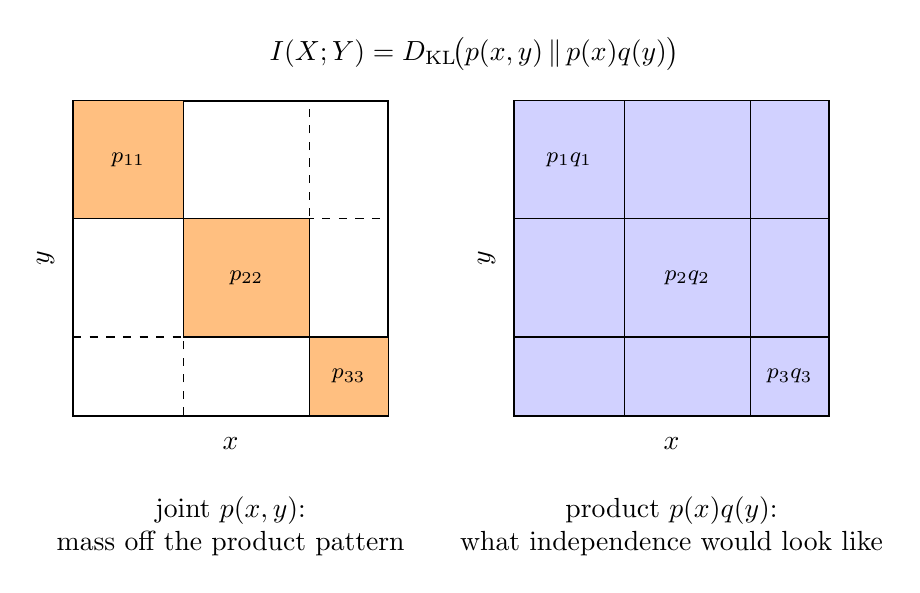
\begin{tikzpicture}[scale=1.0]
% unit square = p(x,y) mass; independent bands vs correlated mass
\draw[thick] (0,0) rectangle (4,4);
\draw[dashed] (0,1) -- (4,1); \draw[dashed] (0,2.5) -- (4,2.5);
\draw[dashed] (1.4,0) -- (1.4,4); \draw[dashed] (3,0) -- (3,4);
\node[rotate=90] at (-0.35,2) {$y$};
\node at (2,-0.35) {$x$};
% correlated mass concentrated near diagonal blocks
\draw[fill=orange!50] (0,2.5) rectangle (1.4,4);
\draw[fill=orange!50] (1.4,1) rectangle (3,2.5);
\draw[fill=orange!50] (3,0) rectangle (4,1);
\node[font=\footnotesize] at (0.7,3.25) {$p_{11}$};
\node[font=\footnotesize] at (2.2,1.75) {$p_{22}$};
\node[font=\footnotesize] at (3.5,0.5) {$p_{33}$};
\begin{scope}[xshift=5.6cm]
  \draw[thick] (0,0) rectangle (4,4);
  \draw[dashed] (0,1) -- (4,1); \draw[dashed] (0,2.5) -- (4,2.5);
  \draw[dashed] (1.4,0) -- (1.4,4); \draw[dashed] (3,0) -- (3,4);
  \foreach \i/\a/\b in {0/0/1.4, 1/1.4/3, 2/3/4}{
    \foreach \j/\c/\d in {0/0/1, 1/1/2.5, 2/2.5/4}{
      \draw[fill=blue!18] (\a,\c) rectangle (\b,\d);}}
  \node[font=\footnotesize] at (0.7,3.25) {$p_1 q_1$};
  \node[font=\footnotesize] at (2.2,1.75) {$p_2 q_2$};
  \node[font=\footnotesize] at (3.5,0.5) {$p_3 q_3$};
  \node[rotate=90] at (-0.35,2) {$y$};
  \node at (2,-0.35) {$x$};
\end{scope}
\node[below, align=center] at (2,-0.9) {joint $p(x,y)$:\\ mass off the product pattern};
\node[below, align=center] at (7.6,-0.9) {product $p(x)q(y)$:\\ what independence would look like};
\node[align=left] at (5.1,4.6) {$\displaystyle I(X;Y)=
  D_{\mathrm{KL}}\!\big(p(x,y)\,\|\,p(x)q(y)\big)$};
\end{tikzpicture}
